\section{Glatting}
\label{sec:Glatting}
\subsection{Bakgrunn}
Glatting, også kalt Gaussian Blur\cite{wiki:blur}, er en veldig mye brukt teknikk innenfor bildebehandling. Man glatter et bilde for å fjerne støy og redusere detaljene i bildet og kan sammenlignes med effekten man får av å se på et bilde gjennom en skjerm som er nesten helt gjennomsiktig. Metoden går essensielt ut på å erstatte verdien i hver piksel med en vektet sum som følger normalfordelingen av pikslene rundt\cite{wiki:blurSV}. 

\subsection{Implementasjon}
\subsubsection{Eksplisitt}
Det eksplisitte skjemaet gitt ved likning (\ref{eq:eksplisitt}) kan løses ved at man tar man utgangspunkt i originalbildet $u_0$ og itererer dette med likning (\ref{eq:diffusjon}) i hele $\Omega$. Bildet \texttt{im} leses derfor inn ved bruk av \texttt{imageio.imread}\footnote{\url{https://pypi.org/project/imageio/}}, før det legges litt støy på bildet.
\begin{lstlisting}[language=Python]
    im = im + .05 * np.random.randn(* np.shape(im))
\end{lstlisting}
Bildet \texttt{im} sendes til \texttt{eksplisittGlatting()} sammen med originalbildet  \texttt{orig\_im} og en konstant k. Her blir det i for-løkka som itereres 20 ganger funnet en laplace for bildet \texttt{image}
\begin{lstlisting}[language=Python]
    laplace = (image[0:-2, 1:-1] + 
            image[2:, 1:-1] +
            image[1:-1, 0:-2] +
            image[1:-1, 2:] -
            4 * image[1:-1, 1:-1])
\end{lstlisting}
For å ha mer kontroll over hvor mye bildet glattes benyttes ``data attachement''. Dette vil si at $h$ settes lik $\lambda(u-u_0)$. 
\begin{lstlisting}[language=Python]
    h = k * delta_t * (image[1:-1, 1:-1] - orig_im[1:-1, 1:-1])
\end{lstlisting}
Da kan det ved å justere parameteren $\lambda$ styres hvor glatt bildet maksimalt kan bli selv om det iteres i det uendelige. Som randverdier brukes Neumann med $\frac{\partial u} {\partial} = 0$ på $\partial \Omega$. Når en itererer likning (\ref{eq:diffusjon}) vil noen verdier kunne gå ut av lovlig intervall, det vil si over 1 eller under 0. Derfor er siste ledd i før-løkka å klippe verdiene i \texttt{image} til et lovlig intervall.
\begin{lstlisting}[language=Python]
    image[image < 0] = 0
    image[image > 1] = 1
\end{lstlisting}
Tilslutt returnes det glattede bildet som vist i Figur \ref{fig:glattingEks}
\begin{figure}
\begin{center}
    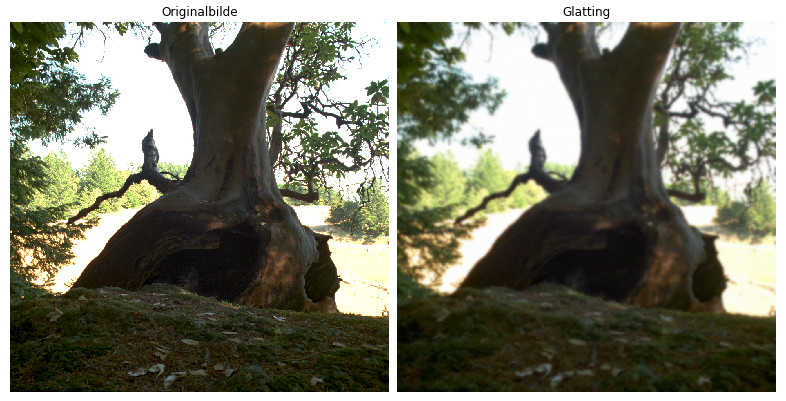
\includegraphics[width=1\columnwidth]{bilder/glattingEksplisitt.jpg}
    \caption{Glatting~ \label{fig:glattingEks}}
\end{center}
\end{figure}

\subsubsection{Implisitt}
\begin{figure}
\begin{center}
    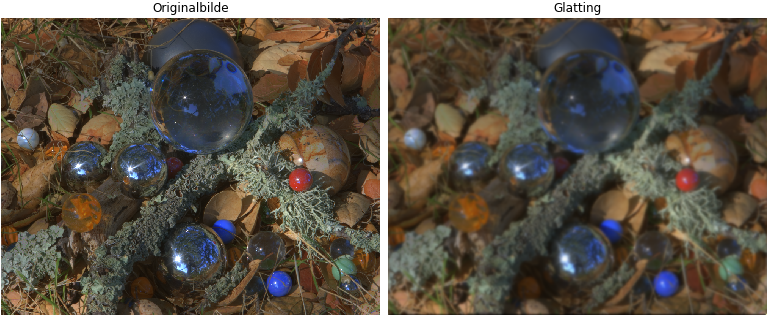
\includegraphics[width=1\columnwidth]{bilder/impGlatt.png}
    \caption{Implisitt glatting med $\alpha=2, n=3$~ \label{fig:glattingImp}}
\end{center}
\end{figure}
For å implementere det implisitte skjemaet gitt ved (\ref{eq:implisitt}) brukes ``sparse matrices''\footnote{\url{https://docs.scipy.org/doc/scipy/reference/sparse.html}}. Her er de aller fleste elementene i matrisa \texttt{0}, bortsett fra noen utvalgte diagonaler. I dette tilfellet får vi en tridiagonal matrise, pluss to ekstra diagonaler. Dersom \texttt{u} er bildet som leses inn, befinner de siste to diagonalene seg henholdsvis \texttt{u.shape[1]} til høyre og venstre for senterdiagonalen. Ved å omskrive (\ref{eq:implisitt}) og sette $\frac{\Delta t}{\Delta x^2} = \alpha$ får vi med \texttt{h=0}:
\begin{align}
    -\alpha u^{n+1}_{i+1,j} 
    -\alpha u^{n+1}_{i-1,j}
    + (1+4\alpha)u^{n+1}_{i,j}
    -\alpha u^{n+1}_{i,j+1}
    -\alpha u^{n+1}_{i,j-1}
    &= u^{n}_{i,j}.
\end{align}
For å skrive dette på matriseform må en altså bruke glisne matriser. Her blir hovedjobben å lage nevnte diagonaler.
\begin{lstlisting}[language=Python]
    size=u.shape[0]*u.shape[1]
    nupper = np.concatenate((np.zeros(u.shape[1]), 
                            -alpha * np.ones(size - u.shape[1])))
    upper = np.concatenate(([0, 0],
                            -alpha * np.ones(size - 2)))
    center = np.concatenate(([1],
                            (1 + 4 * alpha) * np.ones(size - 2),
                            [1]))
    lower = np.concatenate((-alpha * np.ones(size - 2),
                            [0, 0]))
    nlower = np.concatenate((-alpha * np.ones(size - u.shape[1]),
                            np.zeros(u.shape[1])))
    diags = np.array([nupper, upper, center, lower, nlower])
    A = spdiags(diags, [u.shape[1], 1, 0, -1, -u.shape[1]], size, size).tocsc()
\end{lstlisting}
\texttt{nupper} og \texttt{nlower} posisjoneres riktig utfra bildets dimensjoner, mens de tre midterste diagonalene plasseres i midten. Deretter lages en array \texttt{diags} av alle diagonalene. Til slutt settes de sammen til en glissen matrise ved hjelp av \texttt{spdiags()}. I tillegg gjøres de kolonnesentrert med \texttt{tocsc()}.
Denne glissne koeffisientmatrisen \texttt{A} brukes videre i spsolve\footnote{\url{https://docs.scipy.org/doc/scipy-0.14.0/reference/generated/scipy.sparse.linalg.spsolve.html}} som dersom \texttt{u} og \texttt{im} er fargebilder, løser det lineære likningssystemet for hver fargekanal.
\begin{lstlisting}[language=Python]
    for i in range (u.shape[2]):
        im[:,:,i]=spsolve(A,im[:,:,i].flatten()).reshape(u[:,:,i].shape)
\end{lstlisting}
\texttt{flatten()} brukes her for å lage en [1, m $\times$ n] - vektor, der størrelsen på bildet \texttt{u} er m $\times$ n. Ved å bruke et implisitt skjema kontra et eksplisitt, vil en være mindre utsatt for numerisk ustabilitet. Man kan dermed benytte seg av færre iterasjoner og større tidsskritt. I vår implementasjon derimot, opplevde vi at kjøretiden ble langt lenger med implisitt skjema, og de fleste anvendelser benytter derfor det eksplisitte. Figur \ref{fig:glattingImp} viser glatting med implisitt skjema. Her er det brukt 3 iterasjoner, $\alpha$=2 og \texttt{h=0}